

\begin{center}
\thispagestyle{empty}
%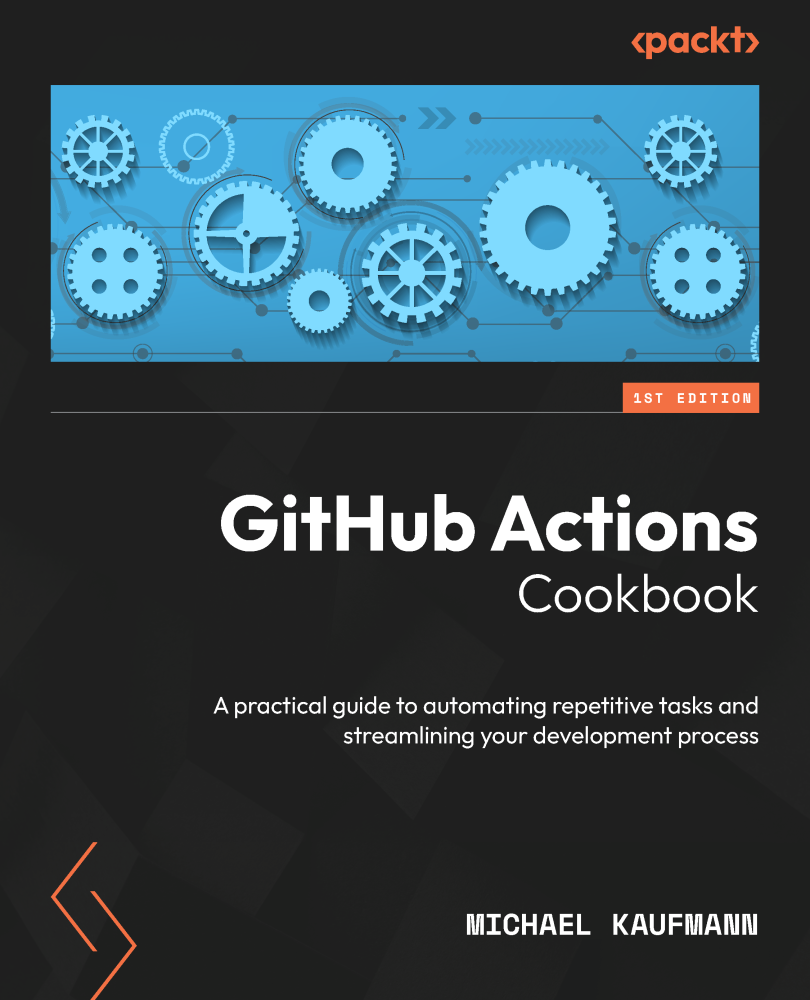
\includegraphics[width=\textwidth,height=\textheight,keepaspectratio]{cover.png}
\begin{tikzpicture}[remember picture, overlay, inner sep=0pt]
\node at (current page.center)
{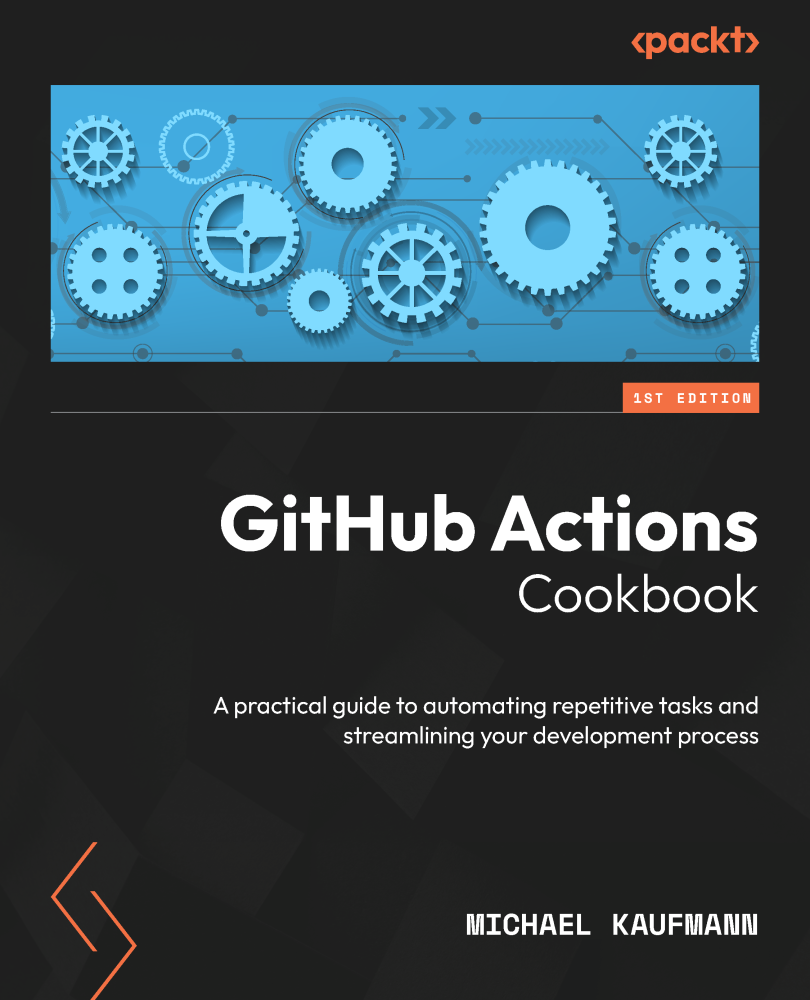
\includegraphics[width=\paperwidth, keepaspectratio=false]{cover.png}};
\end{tikzpicture}
\newpage
\thispagestyle{empty}
\huge
\textbf{GitHub Actions Cookbook}
\\[9pt]
\normalsize
A practical guide to automating repetitive tasks and streamlining your development process
\\[9pt]
\normalsize
作者: Michael Kaufmann
\\[8pt]
\normalsize
译者:\href{https://github.com/xiaoweiChen/GitHub-Actions-Cookbook}{陈晓伟}
\\[8pt]
\end{center}

\newpage

\begin{comment}
\end{comment}

\pagestyle{empty}
\tableofcontents
\newpage

\setsecnumdepth{section}

\myChapter{关于作者}{}{content/about-the-author.tex}
\newpage

\myChapter{前言}{}{content/preface.tex}
\newpage

\myChapter{第1章}{GitHub动作工作流}{content/chapter1/0.tex}
\mySubsection{1.1.}{技术要求}{content/chapter1/1.tex}
\mySubsection{1.2.}{GitHub生态系统}{content/chapter1/2.tex}
\mySubsection{1.3.}{Github的托管和定价}{content/chapter1/3.tex}
\mySubsection{1.4.}{GitHub Actions的价格}{content/chapter1/4.tex}
\mySubsection{1.5.}{GitHub 市场}{content/chapter1/5.tex}
\mySubsection{1.6.}{使用工作流编辑器编写工作流}{content/chapter1/6.tex}
\mySubsection{1.7.}{使用secrets 和 variables}{content/chapter1/7.tex}
\mySubsection{1.8.}{创建和使用环境}{content/chapter1/8.tex}
\newpage

\myChapter{第2章}{编写和调试工作流}{content/chapter2/0.tex}
\mySubsection{2.1.}{使用Visual Studio Code编写工作流}{content/chapter2/1.tex}
\mySubsection{2.2.}{在分支机构开发工作流程}{content/chapter2/2.tex}
\mySubsection{2.3.}{Linting 工作流程}{content/chapter2/3.tex}
\mySubsection{2.4.}{将消息写入日志}{content/chapter2/4.tex}
\mySubsection{2.5.}{启用调试记录}{content/chapter2/5.tex}
\mySubsection{2.6.}{本地运行您的工作流程}{content/chapter2/6.tex}
\newpage

\myChapter{第3章}{构建 GitHub Actions}{content/chapter3/0.tex}
\mySubsection{3.1.}{技术要求}{content/chapter3/1.tex}
\mySubsection{3.2.}{创建Docker容器操作}{content/chapter3/2.tex}
\mySubsection{3.3.}{添加输出参数并使用作业总结}{content/chapter3/3.tex}
\mySubsection{3.4.}{创建一个 TypeScript 动作}{content/chapter3/4.tex}
\mySubsection{3.5.}{创建一个复合动作}{content/chapter3/5.tex}
\mySubsection{3.6.}{在复合操作中使用 github-script 为issue添加评论}{content/chapter3/6.tex}
\mySubsection{3.7.}{将操作共享到市场}{content/chapter3/7.tex}
\newpage

\myChapter{第4章}{The Workflow Runtime}{content/chapter4/0.tex}
\mySubsection{4.1.}{技术要求}{content/chapter4/1.tex}
\mySubsection{4.2.}{Setting up a self-hosted runne}{content/chapter4/2.tex}
\mySubsection{4.3.}{Auto-scaling self-hosted runners}{content/chapter4/3.tex}
\mySubsection{4.4.}{Scaling self-hosted runners with Kubernetes using ARC}{content/chapter4/4.tex}
\mySubsection{4.5.}{Runners and runner groups}{content/chapter4/5.tex}
\mySubsection{4.6.}{GitHub-hosted runners}{content/chapter4/6.tex}
\newpage

\myChapter{第5章}{Automate Tasks in GitHub with GitHub Actions}{content/chapter5/0.tex}
\mySubsection{5.1.}{技术要求}{content/chapter5/1.tex}
\mySubsection{5.2.}{Creating an issue template}{content/chapter5/2.tex}
\mySubsection{5.3.}{Using the GitHub CLI and GITHUB\_TOKEN to access resources}{content/chapter5/3.tex}
\mySubsection{5.4.}{Using environments for approvals and checks}{content/chapter5/4.tex}
\mySubsection{5.5.}{Reusable workflows and composite actions}{content/chapter5/5.tex}
\newpage

\myChapter{第6章}{Build and Validate Your Code}{content/chapter6/0.tex}
\mySubsection{6.1.}{技术要求}{content/chapter6/1.tex}
\mySubsection{6.2.}{Building and testing your code}{content/chapter6/2.tex}
\mySubsection{6.3.}{Building different versions using a matrix}{content/chapter6/3.tex}
\mySubsection{6.4.}{Informing the user on details of your build and test results}{content/chapter6/4.tex}
\mySubsection{6.5.}{Finding security vulnerabilities with CodeQL}{content/chapter6/5.tex}
\mySubsection{6.6.}{Creating a release and publishing the package}{content/chapter6/6.tex}
\mySubsection{6.7.}{Versioning your packages}{content/chapter6/7.tex}
\mySubsection{6.8.}{Generating and using SBOMs}{content/chapter6/8.tex}
\mySubsection{6.9.}{Using caching in workflows}{content/chapter6/9.tex}
\newpage

\myChapter{第7章}{Release Your Software with GitHub Actions}{content/chapter7/0.tex}
\mySubsection{7.1.}{技术要求}{content/chapter7/1.tex}
\mySubsection{7.2.}{Building and publishing a container}{content/chapter7/2.tex}
\mySubsection{7.3.}{Using OIDC to securely deploy to any cloud}{content/chapter7/3.tex}
\mySubsection{7.4.}{Environment approval checks}{content/chapter7/4.tex}
\mySubsection{7.5.}{Releasing the container application to AKS}{content/chapter7/5.tex}
\mySubsection{7.6.}{Automating the update of your dependencies}{content/chapter7/6.tex}
\mySubsection{7.7.}{Clean up}{content/chapter7/7.tex}
\mySubsection{7.8.}{Summary}{content/chapter7/8.tex}
\newpage

\begin{comment}
\end{comment}
